\section{RESULTS}
\label{sec:results}

\begin{figure*}
    \centering
    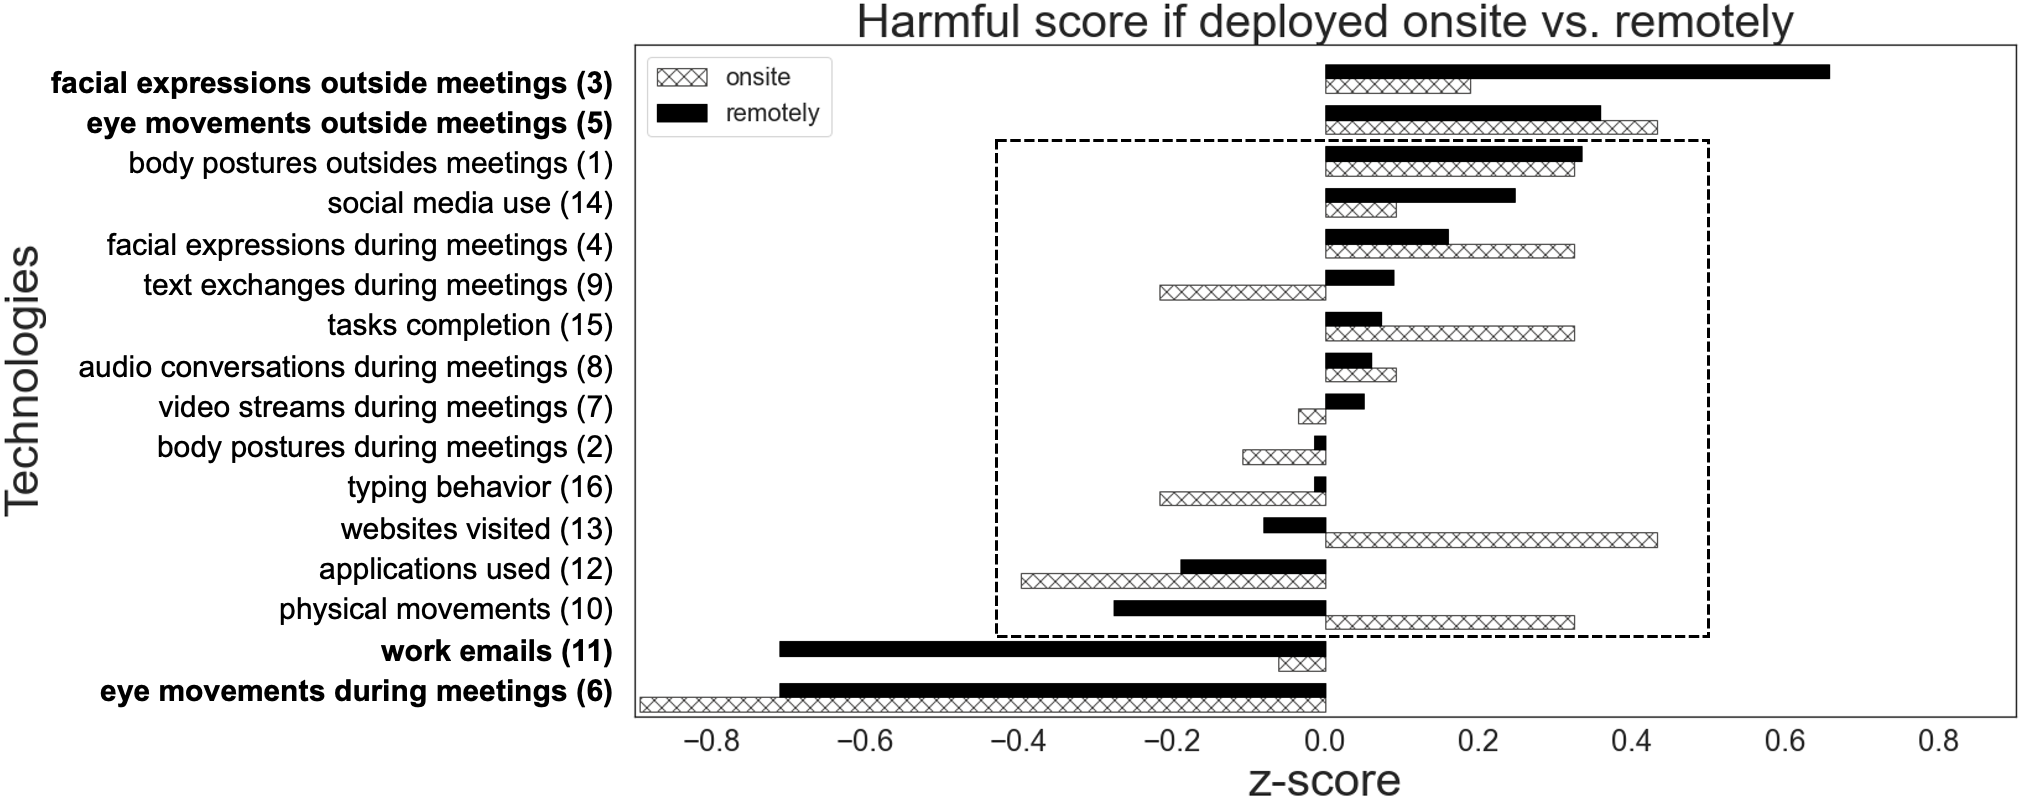
\includegraphics[width=0.93\textwidth]{figures/harm_tech_v4.png}
    \caption{Four groups of technologies emerge: \emph{i)} technologies considered harmful (harmless) both onsite and remotely (inside the dashed box), \emph{ii)} technologies considered harmful (harmless) onsite but not remotely, or vice-versa (inside the dashed box), \emph{iii)} technologies considered harmful remotely (top bars outside the dashed box), and \emph{iv)} technologies considered harmless remotely (bottom bars outside the dashed box).
    }
    \label{fig:harmful_quadrant}
\end{figure*}

\begin{table}[t]
    \centering
    \caption{Conditional probabilities of $p(row | column)$.}
    \begin{tabular}{|l l l l|}
        \hline
        & hard to Adopt & Intrusive & Harmful \\  \hline
        hard to Adopt & 1             & 0.25      & 0.43    \\
        Intrusive     & 0.2           & 1         & 0       \\
        Harmful       & 0.6           & 0         & 1       \\
        \hline
    \end{tabular}
    \label{tab:probs}
\end{table}

Unacceptable scenarios - those that were judged to be hard to adopt, intrusive, and harmful - include \emph{tracking physical movements}, especially \emph{onsite}. This scenario was indeed considered to: be not fully supported by current technologies in use (hard to adopt); interfere with work (intrusive); and infringe on one's freedom of movement (harmful).

As for all the scenarios, we tested how each of them was judged along multiple dimensions. To that end, we computed the conditional probability of a scenario that was judged, say, hard to Adopt to be also judged Harmful. This probability is $p(\textrm{Harmful} | \textrm{hard to Adopt}) $, and is equal to 0.6 (Table~\ref{tab:probs}), meaning that if a scenario is hard to adopt is also likely to be considered harmful, but not always, as we shall see next. More generally, the conditional probabilities are computed as:
$$
p(i | j) = \frac{\# \textrm{cases that are i and j}}{\# \textrm{cases that are j}}$$


From these conditional probabilities, we can see that 20\% of the technologies that are hard to adopt are also considered intrusive, and 60\% are also considered harmful; 25\% of the technologies that are intrusive are considered hard to adopt; finally 43\% of the harmful technologies are considered hard to adopt.

By qualitatively analyzing the ways our participants motivated their judgments, we found that these judgments followed three main heuristics (i.e.,  mental shortcuts used to assess the scenarios quickly and efficiently):


\begin{itemize}

    \item[] \textbf{Viability}. The first heuristic we identified was \textbf{whether the scenario can be easily built from existing technologies in a satisfactory manner}. This judgment criterion is associated with the moral dimension of fairness (any prototype of a technology that is hard to build would inevitably fall short and would be ridden with inaccuracies and biases). For example, in an online meeting, accurately \emph{tracking facial expressions} is technically easy to do using webcams. By contrast, \emph{tracking body postures} is still a hard problem because it requires a combination of wearable sensors such as multiple gyroscopes (e.g., a couple on the earphones~\cite{choi2021kairos, kawsar2018earables}, and the other on a smart watch), which ends up producing spurious classifications of body postures. \\

    \item[] \textbf{Non-intrusiveness}. Another heuristic was \textbf{whether the scenario did not interfere with work or, more generally, was fit for purpose.} This judgment criterion was associated with the two moral dimensions of authority (when the technology is invasive and authoritarian) and loyalty (when the technology disrespects one's way of working and, as often mentioned by our respondents, it has been misused). For example, \emph{tracking eye movements in online meetings}, despite being possible, was considered to be unfit for productivity tracking and be ``on the way'' of getting the job done. By contrast, \emph{tracking text messages in collaboration tools} such as Slack was considered to not interfere with work (unobtrusive) and fit for the purpose of tracking productivity (not misused). \\

    \item[]  \textbf{Responsibility}. The final heuristic was \textbf{whether the scenario was considered responsible in that it did not cause any harm, or infringed on any individual rights.} This was associated with the two moral dimensions of harm (when the technology has negative effects on individuals) and purity (when the technology is seen to disrespect one's beliefs). For example, \emph{tracking audio conversations in online meetings} was considered to be possible (viable), and fit for purpose, yet it was considered to be harmful, as it entailed tracking not only whether a meeting took place but also its content.

\end{itemize}

\begin{figure*}
    \centering
    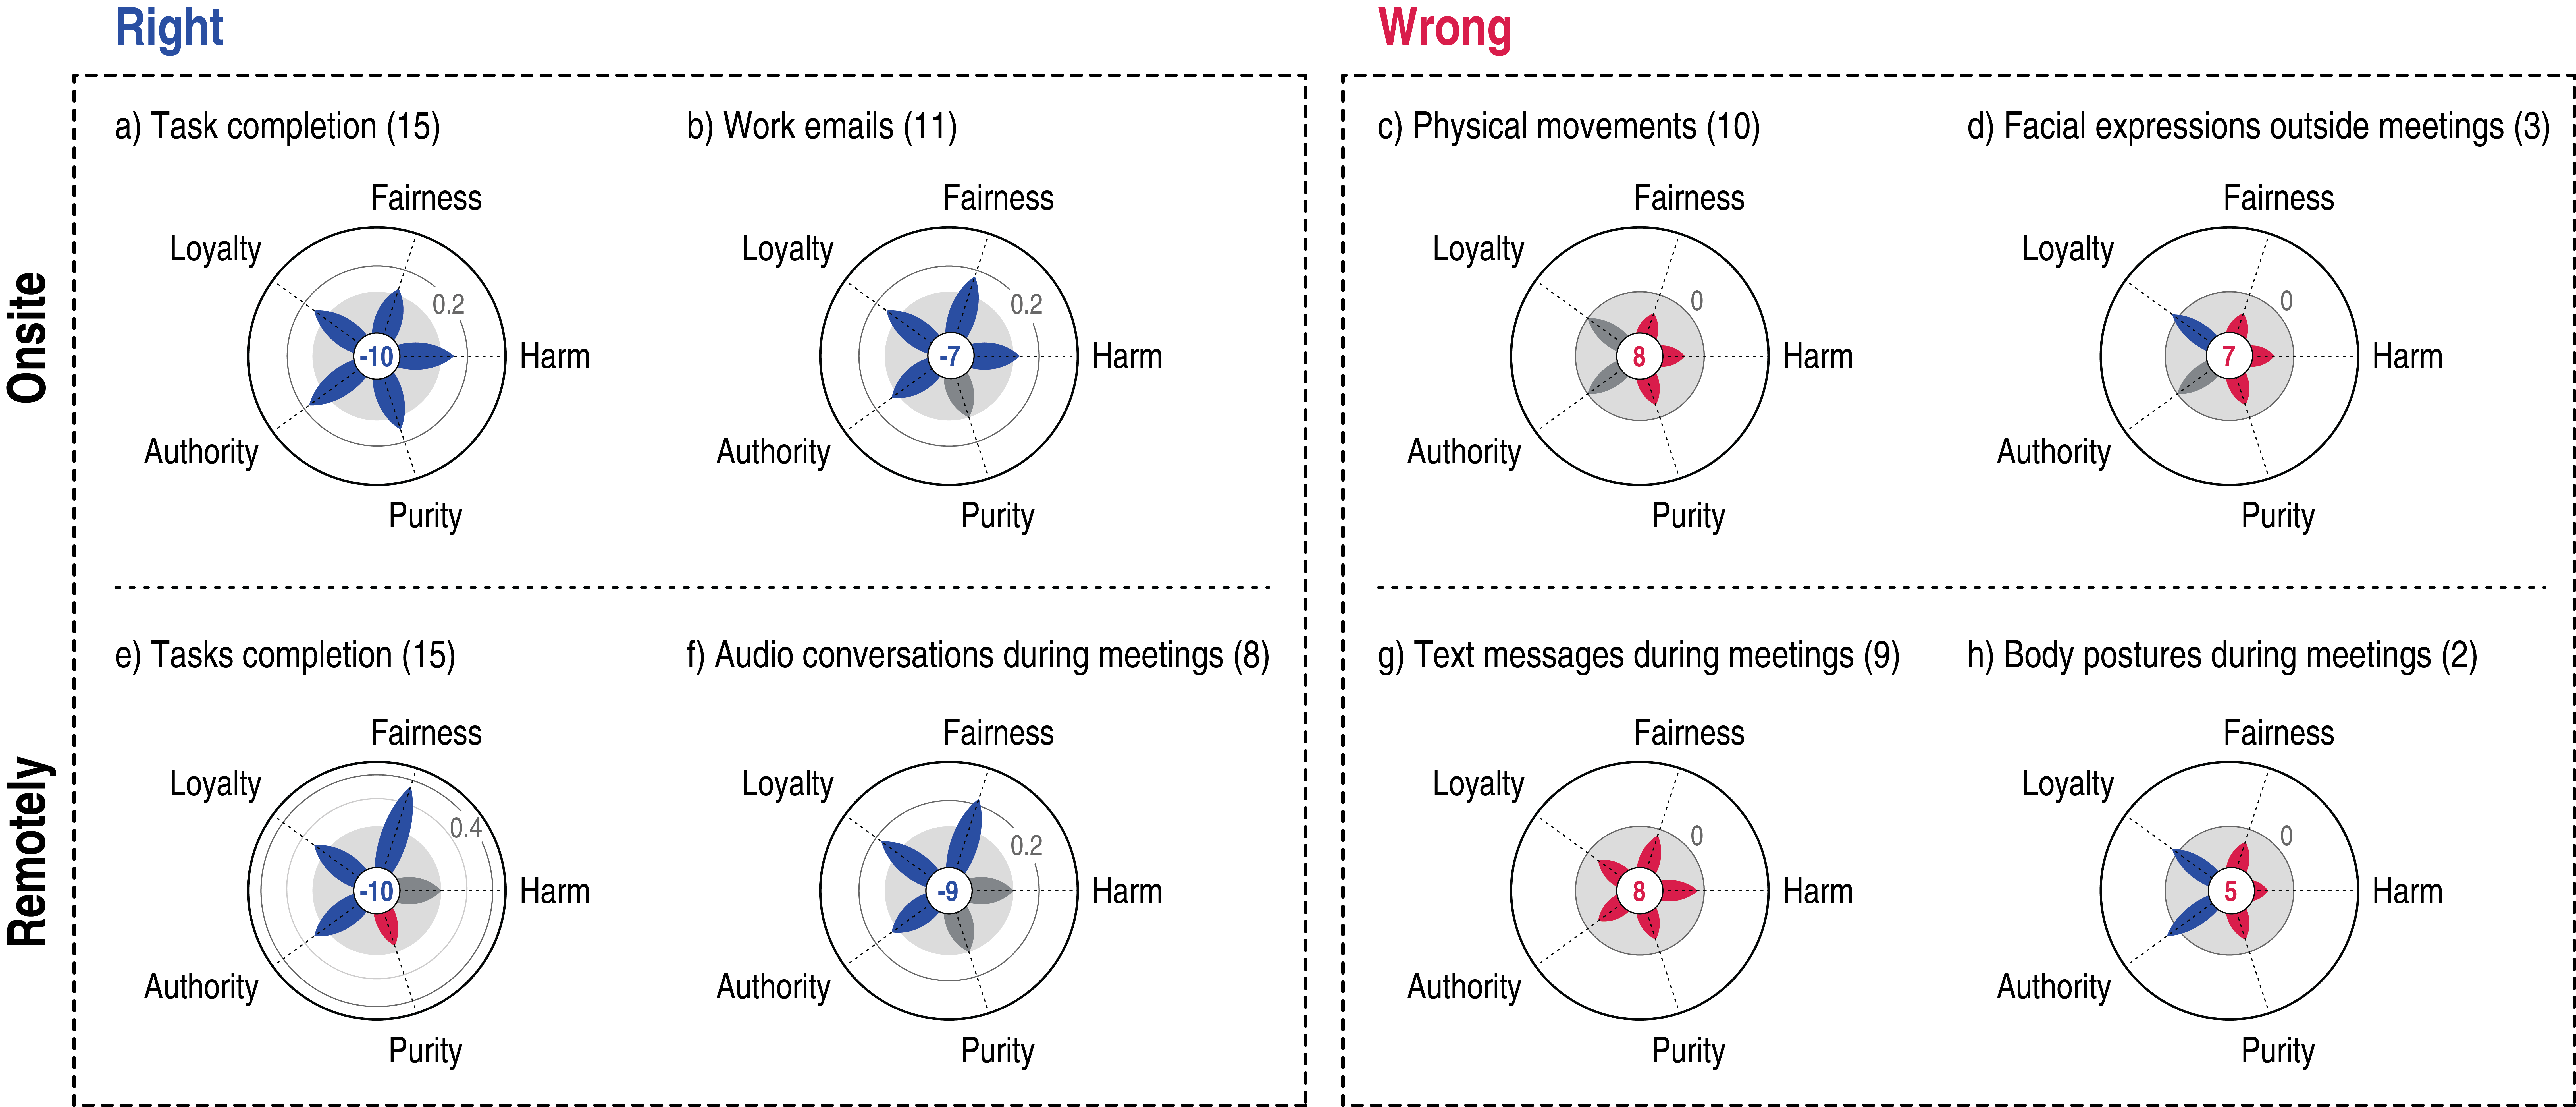
\includegraphics[width=0.92\textwidth]{figures/graphic_v4.png}
    \caption{\textbf{a-b:} Top 2 most ``morally right'' technologies when applied onsite, and \textbf{c-d:} top 2 most ``morally wrong'' technologies when applied onsite. \textbf{e-f:} Top 2 most ``morally right'' technologies when applied remotely, and \textbf{g-h:} top 2 most ``morally wrong'' technologies when applied remotely. Each technology is marked with its number in Table~\ref{tab:technologies} in parenthesis. The wrongness score (showed at the center of each radar plot) was computed by aggregating the negative and the positive words of the individual five moral dimensions (\S\nameref{sec:procedure}), and captures how morally wrong the technology was considered on average to be. Dark blue denotes more positive words associated with a dimension, red denotes more negative words, and gray blue denotes equal amount of positive and negative words.}
    \label{fig:radar_plots}
\end{figure*}

\subsection{Onsite vs. Remotely: Clustering how technologies are judged}
Figure~\ref{fig:harmful_quadrant} shows the harmful score when a technology is deployed onsite versus when it is deployed remotely. Four groups of technologies emerge: \emph{a)} technologies considered harmful (harmless) both onsite and remotely, \emph{b)} technologies considered harmful (harmless) onsite but not remotely, or vice-versa, \emph{c)} technologies considered harmful remotely, and \emph{d)} technologies considered harmless remotely. As for the first two groups of technologies, for example, \emph{tracking audio conversations during meetings} led to same judgments irrespective the deployment setting, while, \emph{tracking text exchanges during meetings} led to opposite judgments. As for the third group, \emph{tracking eye movements} and \emph{facial expressions outside meetings} were considered more harmful when deployed remotely, not least because remote work typically happens in a private space~\cite{nippert2010islands} such as one's home~\cite{rudnicka2020eworklife}, and, as a result, the use of tracking devices should be limited to specific work-related activities and should ideally not go beyond them. As for the fourth group, \emph{tracking work emails} and \emph{tracking eye movements during meetings} were considered less harmful when deployed remotely. As it is harder to measure productivity in remote settings, tracking work emails was considered a reasonable proxy for attention levels and a compromise to accept\footnote{\url{https://www.gartner.com/smarterwithgartner/9-future-of-work-trends-post-covid-19}}\footnote{\url{https://www.computerworld.com/article/3586616/the-new-normal-when-work-from-home-means-the-boss-is-watching.html}}. Also, \emph{tracking eye movements during meetings} was seen as a proxy for body cues (e.g., facial expressions), which could reflect attention levels and often go unnoticed in virtual meetings~\cite{choi2021kairos}.

\subsection{Words associated with moral dimensions}
Next, we looked into how crowd-workers associated our technologies with words related to the five moral dimensions of \emph{harm, fairness, loyalty, authority, and purity}. We computed the fraction of times a word associated with each moral dimension was chosen (Figure~\ref{fig:radar_plots}). For example, \emph{tracking task completion onsite} (technology 15 in Table~\ref{tab:technologies}) was associated with fairness, loyalty, authority, purity, and lack of harm. The very same technology though when applied remotely was again associated with fairness, loyalty, authority, but also with harm and lack of purity.

By aggregating the negative and the positive words of the five moral dimensions (as per signs in \S\nameref{sec:procedure}), we computed a scenario's `wrongness'. This score captures how morally wrong or right a technology is. Technologies that were considered to be morally right (blue in Figure~\ref{fig:radar_plots}) were associated with positive words (e.g., fair, impartial), while those considered to be morally wrong (red in Figure~\ref{fig:radar_plots}) were associated with negative words (e.g., unjust, discriminatory). We found that morally right technologies with negative values of wrongness in Figures~\ref{fig:radar_plots}a-b, and Figures~\ref{fig:radar_plots}e-f were those that track productivity based on task completion, work emails, and audio and textual conversations during meetings, whereas morally wrong technologies (Figure~\ref{fig:radar_plots}c-d, and g-h) were those that involved some kind of body-tracking such as tracking physical movements and facial expressions. 